% Gemini theme
% https://github.com/anishathalye/gemini

\documentclass[final]{beamer}

% ====================
% Packages
% ====================

\usepackage[T1]{fontenc}
\usepackage{lmodern}
\usepackage[size=custom,width=120,height=72,scale=1.0]{beamerposter}
\usetheme{gemini}
\usecolortheme{mit}
\usepackage{graphicx}
\usepackage{booktabs}
\usepackage{bchart}
\usepackage{tikz}
\usepackage{pgfplots}
\pgfplotsset{compat=1.14}
\usepackage{anyfontsize}
\usepackage{multicol}
\usepackage{xcolor}
% ====================
% Lengths
% ====================

% If you have N columns, choose \sepwidth and \colwidth such that
% (N+1)*\sepwidth + N*\colwidth = \paperwidth
\newlength{\sepwidth}
\newlength{\colwidth}
\setlength{\sepwidth}{0.025\paperwidth}
\setlength{\colwidth}{0.3\paperwidth}

\newcommand{\separatorcolumn}{\begin{column}{\sepwidth}\end{column}}

% ====================
% Title
% ====================

\title{Estrategias para la exploración coordinada multi-VANT}

\author{Luis Alberto Ballado Aradias \and Dr. José Gabriel Ramirez-Torres \and Dr. Eduardo Arturo Rodriguez-Tello}

\institute[shortinst]{CINVESTAV - UNIDAD TAMAULIPAS}

% ====================
% Footer (optional)
% ====================

\footercontent{
  \href{https://www.tamps.cinvestav.mx/}{https://www.tamps.cinvestav.mx/} \hfill
  CINVESTAV UNIDAD TAMAULIPAS 2023 \hfill
  \href{mailto:luis.ballado@cinvestav.mx}{luis.ballado@cinvestav.mx}}
% (can be left out to remove footer)

% ====================
% Logo (optional)
% ====================

% use this to include logos on the left and/or right side of the header:
\logoright{
\includegraphics[height=7cm]{logoCinves.png}}
\logoleft{
\includegraphics[height=7cm]{cinves.png}}

% ====================
% Body
% ====================

\begin{document}

\begin{frame}[t]
\begin{columns}[t]
\separatorcolumn
\begin{column}{\colwidth}
  \begin{block}{\color{teal}\textbf{Vehículos Aéreos No Tripulados Estadísticas}}

    Los Vehículos Aéreos No Tripulados (VANTS), han experimentado un rápido crecimiento en los últimos años. Su versatilidad y capacidad para acceder a áreas de difícil acceso han impulsado su adopción en diferentes sectores.
    A medida que la tecnología continúa avanzando, se espera que los drones autónomos desempeñen un papel cada vez más importante en áreas como la inteligencia artificial y la integración en la vida cotidiana.\cite{shannon1948communication}\\
    
    \begin{multicols}{2}
      \begin{figure}[h]
        \hspace*{-2.5cm} 
      \scalebox{0.9}{
        \begin{tikzpicture}
          \begin{axis}[title  = \textbf{Valuación Soluciones 2020 Billones-USD},
              xbar,
              y axis line style = { opacity = 0 },
              axis x line       = none,
              tickwidth         = 0pt,
              ytick             = data,
              enlarge y limits  = 0.05,
              enlarge x limits  = 0.02,
              width=0.45\textwidth,
              bar width=6mm,
              symbolic y coords = {Infraestructura, Agricultura, Transporte, Seguridad, Entretenimiento, Seguros, Telecomunicaciones, Mineria},
              nodes near coords,
            ]
            \addplot coordinates { (45.2,Infraestructura) (32.4,Agricultura) (13,Transporte) (10,Seguridad) (8.8,Entretenimiento) (6.8,Seguros) (6.3,Telecomunicaciones) (4.4,Mineria)};
          \end{axis}
        \end{tikzpicture}
      }
    \end{figure}
    
      \begin{figure}[t]
        \hspace*{1cm} 
      \begin{tikzpicture}
        \begin{axis}[title  = \textbf{Artículos VANTS},
	    x tick label style={
	      /pgf/number format/1000 sep=},
	    ylabel=Artículos,
	    enlargelimits=0.05,
            width=0.45\textwidth,
	    legend style={at={(0.5,-0.1)},
	      anchor=north,legend columns=-1},
	    ybar interval=0.7,
          ]
          \addplot 
	  coordinates {(16,110) (17,150) (18,246) (19,392) (20,634) (21,995) (22,1414) (23,1929) (24,2329)};
        \end{axis}
      \end{tikzpicture}
    \end{figure}
    \end{multicols}
  \end{block}
  
  \begin{block}{\color{teal}Robot Autónomo}
    %\heading{Another heading inside a block}
    Los robots autónomos representan una fascinante frontera en la robótica y la inteligencia artificial, ya que deben poseer la capacidad de tomar decisiones y ejecutar tareas de manera independiente.
    \begin{figure}
      \centering
      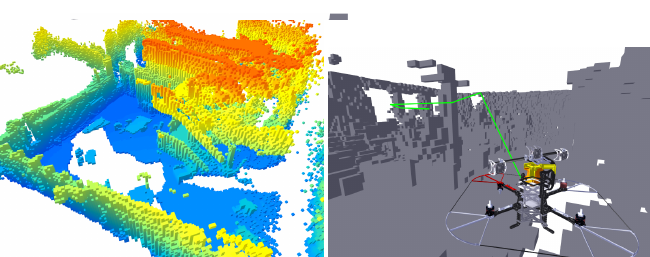
\includegraphics[width=40cm]{images/auto_dro.png}
    \end{figure}

    Para que un robot sea considerado autónomo, debe responder las siguientes preguntas:
    \begin{multicols}{3}
      \begin{itemize}
      \item \textbf{¿Dónde estoy?}\\
        Sensores avanzados como cámaras y lidar, permiten conocer su entorno.\\
        Esta conciencia espacial les permite adaptarse dinámicamente y ubicarse en su entorno.\vspace{1cm}
      \item \textbf{¿A dónde voy?}\\
        Capacidad de determinar una dirección futura se basa en algoritmos de planificación y toma de decisiones, considerando variables como obstáculos y restricciones del entorno.\vspace{1cm}
      \item \textbf{¿Cómo llego ahí?}\\
        La percepción, planificación y ejecución de sus movimientos, permite adaptarse a entornos dinámicos y superar obstáculos de manera autónoma.
      \end{itemize}
    \end{multicols}
  \end{block}
\end{column}

\separatorcolumn

\begin{column}{\colwidth}
  
  \begin{block}{\color{teal}VANT tipo Multi-rotor}
    \begin{enumerate}
      \item \textbf{Sensores de Percepción}. Incluyen cámaras, lidar, entre otros, que permiten al VANT recopilar información sobre su entorno.
      \item \textbf{Sistema de Control}. Contiene el procesador y los algoritmos que permiten al VANT tomar decisiones autónomas basadas en la información recopilada por los sensores.
      \item \textbf{Sistema de Propulsión}, Los motores y las hélices proporcionan la fuerza necesaria para el vuelo. La configuración de los motores puede variar según su capacidad de maniobra.
    \end{enumerate}

    \begin{figure}[t]
      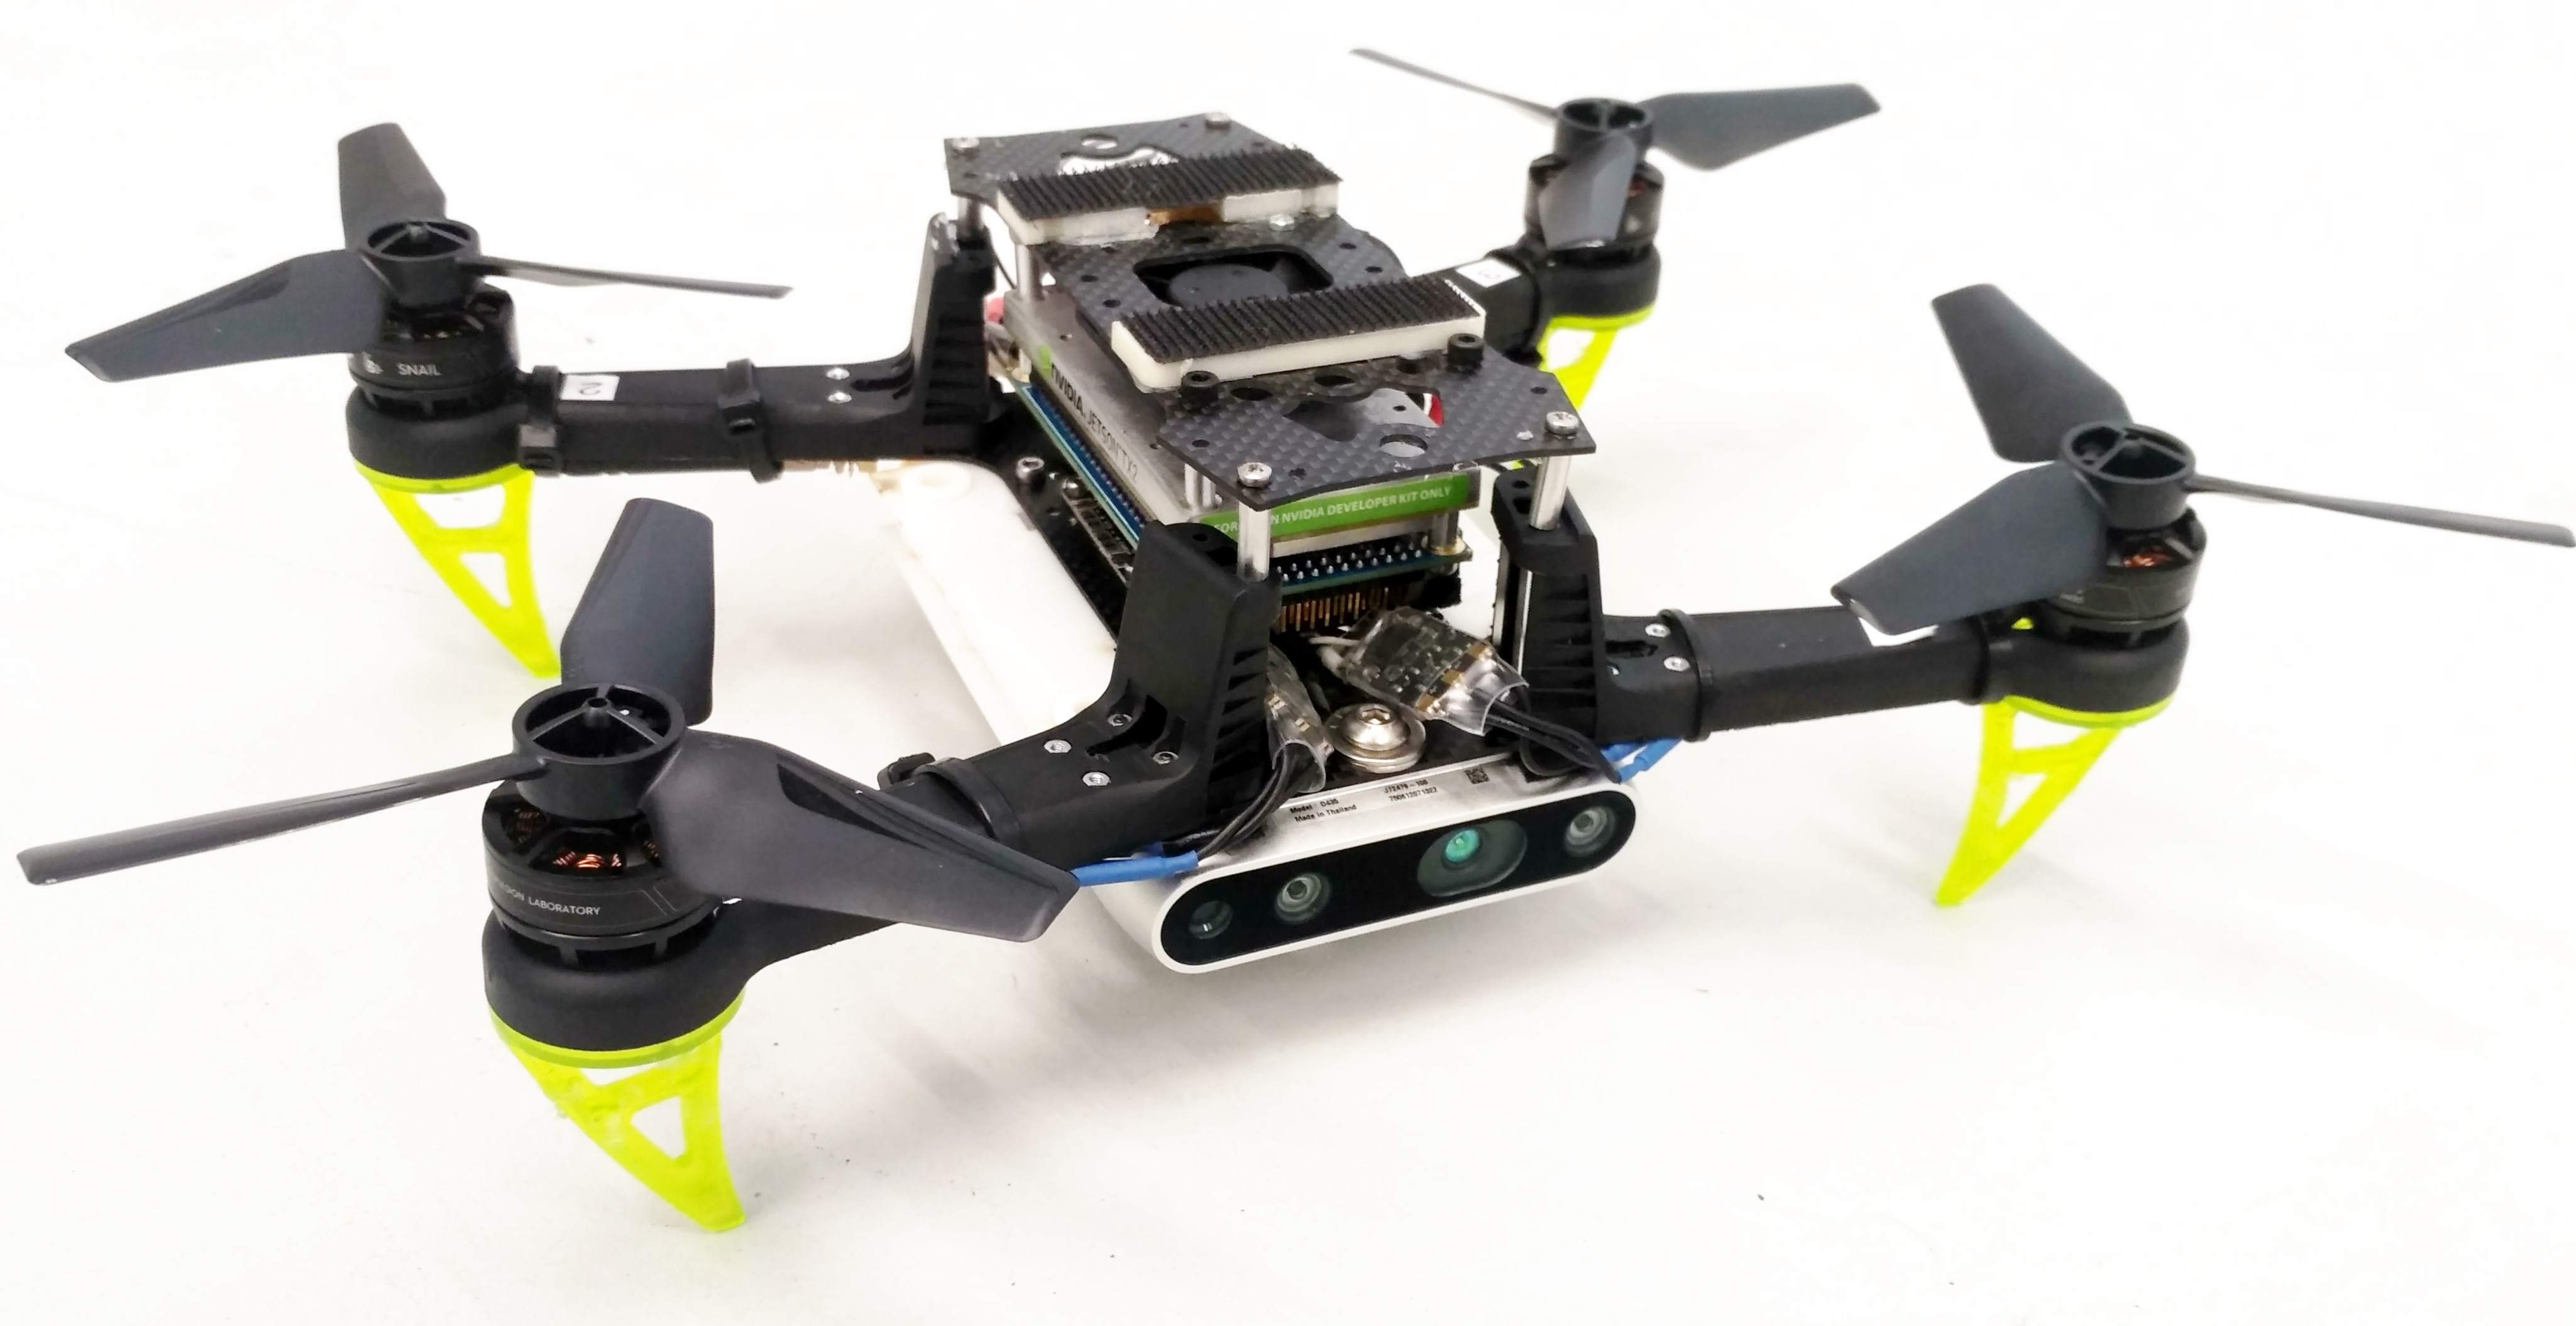
\includegraphics[width=30cm]{images/uav_planning_drone.jpg}
      \centering
    \end{figure}
    
  \end{block}
  
  \begin{block}{\color{teal}Arquitectura Exploración}
    Exploración es una tarea fundamental en robots autónomos. El objetivo es crear un mapa de un ambiente desconocido.
    \begin{figure}[t]
      \centering
      
\includegraphics[width=32cm]{images/exploracion.png}
    \end{figure}
    
    \begin{itemize}
    \item \textbf{Sensor} Incluyen cámaras, lidar, entre otros, que permiten al VANT recopilar información sobre su entorno.
    \item \textbf{Creación Mapa} Incluyen cámaras, lidar, entre otros, que permiten al VANT recopilar información sobre su entorno.
    \item \textbf{Localización} Incluyen cámaras, lidar, entre otros, que permiten al VANT recopilar información sobre su entorno.
    \item \textbf{Exploración} Incluyen cámaras, lidar, entre otros, que permiten al VANT recopilar información sobre su entorno.
    \item \textbf{Planificación trayectoria} Incluyen cámaras, lidar, entre otros, que permiten al VANT recopilar información sobre su entorno.
    \item \textbf{Control} Incluyen cámaras, lidar, entre otros, que permiten al VANT recopilar información sobre su entorno.
    \end{itemize}
  \end{block}
\end{column}

\separatorcolumn

\begin{column}{\colwidth}
  
  \begin{block}{\color{teal}Aplicaciones}

    \begin{figure}
      \centering
      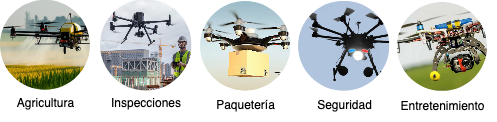
\includegraphics[width=30cm]{images/ap_dr.png}
      \end{figure}
  \end{block}

  \begin{block}{\color{teal}Estrategia exploración coordinada}

    \begin{figure}
      \centering
      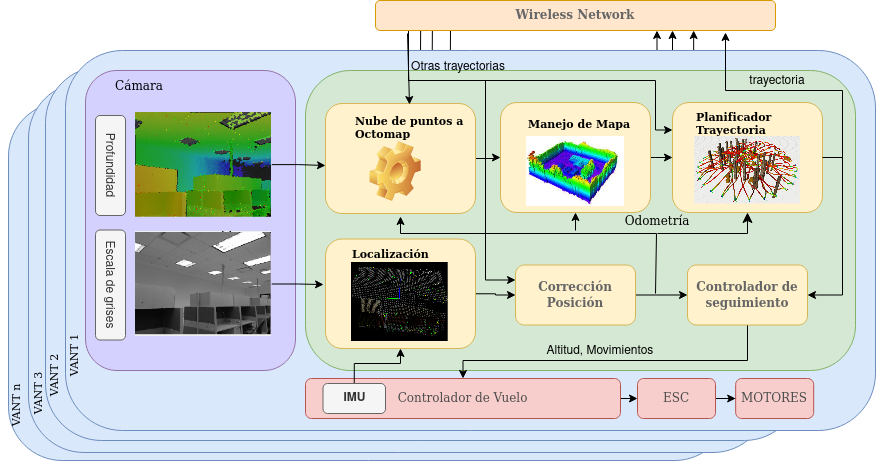
\includegraphics[width=35cm]{images/arquitectura.png}
    \end{figure}

    \begin{figure}
      \centering
      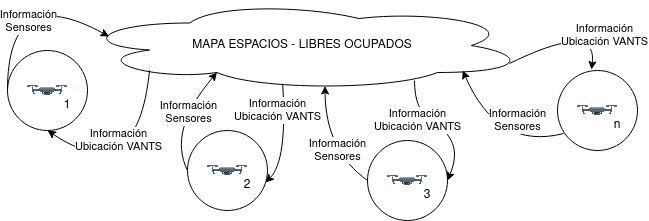
\includegraphics[width=35cm]{images/problema.png}
      \end{figure}
    

  \end{block}

  \begin{block}{\color{teal}Referencias}

    \nocite{*}
    \footnotesize{\bibliographystyle{plain}\bibliography{poster}}

  \end{block}

\end{column}

\separatorcolumn
\end{columns}
\end{frame}

\end{document}
